\documentclass[]{article}
\usepackage{lmodern}
\usepackage{amssymb,amsmath}
\usepackage{ifxetex,ifluatex}
\usepackage{fixltx2e} % provides \textsubscript
\ifnum 0\ifxetex 1\fi\ifluatex 1\fi=0 % if pdftex
  \usepackage[T1]{fontenc}
  \usepackage[utf8]{inputenc}
\else % if luatex or xelatex
  \ifxetex
    \usepackage{mathspec}
  \else
    \usepackage{fontspec}
  \fi
  \defaultfontfeatures{Ligatures=TeX,Scale=MatchLowercase}
\fi
% use upquote if available, for straight quotes in verbatim environments
\IfFileExists{upquote.sty}{\usepackage{upquote}}{}
% use microtype if available
\IfFileExists{microtype.sty}{%
\usepackage{microtype}
\UseMicrotypeSet[protrusion]{basicmath} % disable protrusion for tt fonts
}{}
\usepackage[margin=1in]{geometry}
\usepackage{hyperref}
\hypersetup{unicode=true,
            pdftitle={R Final Report},
            pdfauthor={Chen Ming},
            pdfborder={0 0 0},
            breaklinks=true}
\urlstyle{same}  % don't use monospace font for urls
\usepackage{graphicx,grffile}
\makeatletter
\def\maxwidth{\ifdim\Gin@nat@width>\linewidth\linewidth\else\Gin@nat@width\fi}
\def\maxheight{\ifdim\Gin@nat@height>\textheight\textheight\else\Gin@nat@height\fi}
\makeatother
% Scale images if necessary, so that they will not overflow the page
% margins by default, and it is still possible to overwrite the defaults
% using explicit options in \includegraphics[width, height, ...]{}
\setkeys{Gin}{width=\maxwidth,height=\maxheight,keepaspectratio}
\IfFileExists{parskip.sty}{%
\usepackage{parskip}
}{% else
\setlength{\parindent}{0pt}
\setlength{\parskip}{6pt plus 2pt minus 1pt}
}
\setlength{\emergencystretch}{3em}  % prevent overfull lines
\providecommand{\tightlist}{%
  \setlength{\itemsep}{0pt}\setlength{\parskip}{0pt}}
\setcounter{secnumdepth}{0}
% Redefines (sub)paragraphs to behave more like sections
\ifx\paragraph\undefined\else
\let\oldparagraph\paragraph
\renewcommand{\paragraph}[1]{\oldparagraph{#1}\mbox{}}
\fi
\ifx\subparagraph\undefined\else
\let\oldsubparagraph\subparagraph
\renewcommand{\subparagraph}[1]{\oldsubparagraph{#1}\mbox{}}
\fi

%%% Use protect on footnotes to avoid problems with footnotes in titles
\let\rmarkdownfootnote\footnote%
\def\footnote{\protect\rmarkdownfootnote}

%%% Change title format to be more compact
\usepackage{titling}

% Create subtitle command for use in maketitle
\providecommand{\subtitle}[1]{
  \posttitle{
    \begin{center}\large#1\end{center}
    }
}

\setlength{\droptitle}{-2em}

  \title{R Final Report}
    \pretitle{\vspace{\droptitle}\centering\huge}
  \posttitle{\par}
    \author{Chen Ming}
    \preauthor{\centering\large\emph}
  \postauthor{\par}
      \predate{\centering\large\emph}
  \postdate{\par}
    \date{May 20th}


\begin{document}
\maketitle

\hypertarget{part-1}{%
\section{Part 1}\label{part-1}}

\hypertarget{report-descriptive-statistics-of-the-data-set-obtained-in-a.}{%
\paragraph{\texorpdfstring{\textbf{1.1 Report descriptive statistics of
the data set obtained in (a).
}}{1.1 Report descriptive statistics of the data set obtained in (a). }}\label{report-descriptive-statistics-of-the-data-set-obtained-in-a.}}

The descriptive statistics of the data are summarized in the following
table.

\begin{verbatim}
##      item Wr.Hnd NW.Hnd  Pulse Height   Age
## 1    Min.   13.0  12.50  35.00  152.0 16.92
## 2 1st Qu.   17.5  17.50  66.75  165.0 17.67
## 3  Median   18.5  18.50  72.00  170.6 18.58
## 4    Mean   18.8  18.73  74.02  172.5 20.43
## 5 3rd Qu.   20.0  20.00  80.00  180.0 20.17
## 6    Max.   23.2  23.50 104.00  200.0 70.42
\end{verbatim}

\begin{figure}
\begin{center}
\includegraphics{table.png}
\end{center}
\end{figure}

\hypertarget{use-boxplot-to-show-the-distributions-of-the-height-of-male-and-female-students.}{%
\paragraph{\texorpdfstring{\textbf{1.2 Use boxplot to show the
distributions of the height of male and female
students.}}{1.2 Use boxplot to show the distributions of the height of male and female students.}}\label{use-boxplot-to-show-the-distributions-of-the-height-of-male-and-female-students.}}

The distributions of the height of male and female students are as
follows.
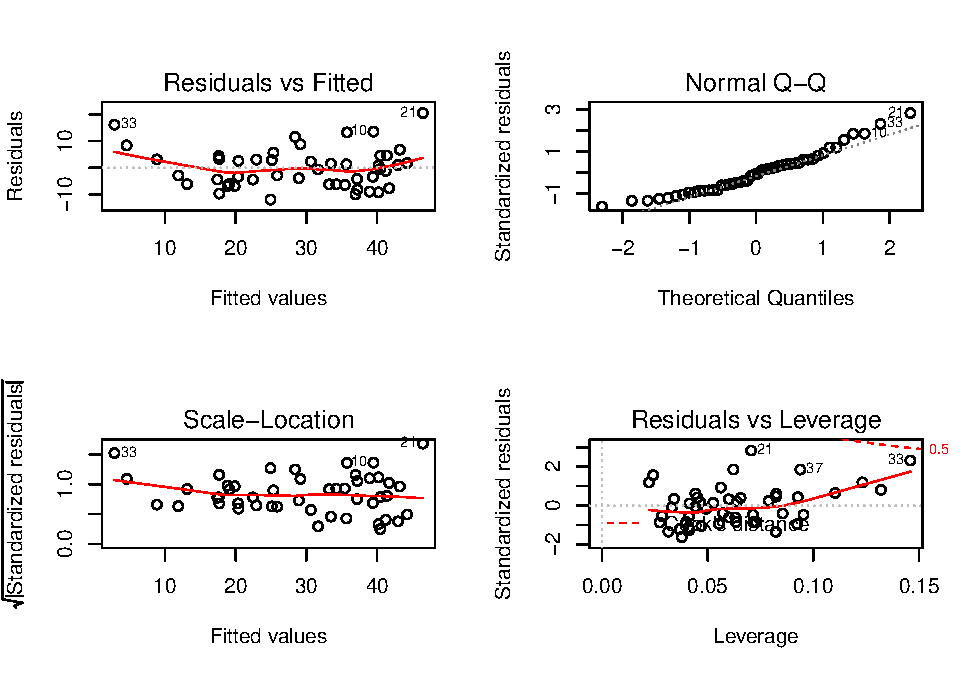
\includegraphics{rmarkdown_for_final_report_files/figure-latex/unnamed-chunk-3-1.pdf}

\hypertarget{which-numerical-variables-might-have-an-influence-on-the-students-pulse}{%
\paragraph{\texorpdfstring{\textbf{1.3 Which numerical variables might
have an influence on the student's pulse?
}}{1.3 Which numerical variables might have an influence on the student's pulse? }}\label{which-numerical-variables-might-have-an-influence-on-the-students-pulse}}

To indentify variables that have influence on students' pulse, we can
conduct regression analysis. By fitting models with ``Pulse'' as
dependent variables and other numerical variables as independent
variables respectively, we can easily find that all the numerical
variables might have an influence on students' pulse, with p-value of
those fitted model all below 0.01.

\hypertarget{is-the-probability-of-a-student-clapping-hisher-left-hand-on-top-less-than-0.2}{%
\paragraph{\texorpdfstring{\textbf{1.4 Is the probability of a student
clapping his/her left hand on top less than 0.2?
}}{1.4 Is the probability of a student clapping his/her left hand on top less than 0.2? }}\label{is-the-probability-of-a-student-clapping-hisher-left-hand-on-top-less-than-0.2}}

To make sure whether the probability of a student clapping hand on top
less than 0.2, we can use \textbf{prop.test} funtion to conduct
proportion test. The null hypothesis is that ``The probability of a
student clapping his/her left hand on top greater than or equal to
0.2'', and the alternative hypothesis is that ``probability of a student
clapping his/her left hand on top less than 0.2''. The result suggests
that the p-value is 0.1626, which means that we cannot reject the null
hypothesis at .1 level of significance. Therefore we can infer that the
probability of a student clapping his/her left hand on top is equal to
or greater than 0.2.

\hypertarget{is-the-span-of-the-writing-hand-in-general-larger-than-the-span-of-the-non-writing-hand}{%
\paragraph{\texorpdfstring{\textbf{1.5 Is the span of the writing hand
in general larger than the span of the non-writing hand?
}}{1.5 Is the span of the writing hand in general larger than the span of the non-writing hand? }}\label{is-the-span-of-the-writing-hand-in-general-larger-than-the-span-of-the-non-writing-hand}}

To make sure whether the span of the writing hand in general larger than
the span of the non-writing hand, we can make a hypothesis test. The
null hypothesis is `the span of the writing hand is in general smaller
than or equal to the span of the non-writing hand', and the alternative
hypothesis is `the span of the writing hand is in general larger to the
span of the non-writing hand'. With a p-value of 0.3696, The hypothesis
test result suggests that we cannot reject the null hypothesis.
Therefore the the span of the writing hand is in general equal to or
smaller than the span of the non-writing hand.

\hypertarget{part-2}{%
\section{Part 2}\label{part-2}}

\hypertarget{according-to-clt-what-is-the-approximated-distribution-of-the-sample-means}{%
\paragraph{\texorpdfstring{\textbf{2.1 According to CLT, what is the
approximated distribution of the sample means?
}}{2.1 According to CLT, what is the approximated distribution of the sample means? }}\label{according-to-clt-what-is-the-approximated-distribution-of-the-sample-means}}

According to CLT, the means of the sample tends towards a normal
distribution. The approximated distribution of the sample means is
normal distribution.

\hypertarget{draw-the-density-plots-of-the-sample-means-and-its-approximated-distribution-on-one-graph.}{%
\paragraph{\texorpdfstring{\textbf{2.2 Draw the density plots of the
sample means and its approximated distribution on one
graph.}}{2.2 Draw the density plots of the sample means and its approximated distribution on one graph.}}\label{draw-the-density-plots-of-the-sample-means-and-its-approximated-distribution-on-one-graph.}}

\includegraphics{rmarkdown_for_final_report_files/figure-latex/unnamed-chunk-9-1.pdf}

\hypertarget{show-the-qq-plot-of-the-distribution-of-the-sample-means.}{%
\paragraph{\texorpdfstring{\textbf{2.3 Show the qq plot of the
distribution of the sample means.
}}{2.3 Show the qq plot of the distribution of the sample means. }}\label{show-the-qq-plot-of-the-distribution-of-the-sample-means.}}

The QQ plot of the distribution of the sample means is as follows.
\includegraphics{rmarkdown_for_final_report_files/figure-latex/unnamed-chunk-10-1.pdf}

\hypertarget{what-conclusion-can-you-draw-from-this-simulation}{%
\paragraph{\texorpdfstring{\textbf{2.4 What conclusion can you draw from
this
simulation?}}{2.4 What conclusion can you draw from this simulation?}}\label{what-conclusion-can-you-draw-from-this-simulation}}

From the density plot, we can know that the sample means distribution
tends towards normal distribution as the sample means number get
greater. From QQ plot, we can also observe that the points fall on the
straight 45-degree line, which suggests that the residual values are
normally distributed with a mean of 0. Hence the sample means are
normally distributed.

\hypertarget{part-3}{%
\section{Part 3}\label{part-3}}

\hypertarget{draw-5000-random-samples-of-x.}{%
\paragraph{\texorpdfstring{\textbf{3.1 Draw 5000 random samples of
X.}}{3.1 Draw 5000 random samples of X.}}\label{draw-5000-random-samples-of-x.}}

The random samples generated are omitted here.

\hypertarget{given-alpha-0.05-find-the-var-of-the-samples-obtained-in-a.}{%
\paragraph{\texorpdfstring{\textbf{3.2 Given \(\alpha\) = 0.05, find the
VaR of the samples obtained in a).
}}{3.2 Given \textbackslash alpha = 0.05, find the VaR of the samples obtained in a). }}\label{given-alpha-0.05-find-the-var-of-the-samples-obtained-in-a.}}

Since VaR denotes the critical value \(L\) such that \(P(X>L)=\alpha\)
,to find the VaR of the samples, we first need to sort the array of the
change of the stock price ascendingly. Then we can use \textbf{quantile}
function to find out the change value situated at given \(\alpha\). The
VaR is -2.130284.

\hypertarget{find-the-cvar-of-the-samples-obtained-in-a.}{%
\paragraph{\texorpdfstring{\textbf{3.3 Find the CVaR of the samples
obtained in a).
}}{3.3 Find the CVaR of the samples obtained in a). }}\label{find-the-cvar-of-the-samples-obtained-in-a.}}

\hypertarget{part-4}{%
\section{Part 4}\label{part-4}}

\hypertarget{report-on-data-exploration.}{%
\paragraph{\texorpdfstring{\textbf{4.1 Report on data
exploration.}}{4.1 Report on data exploration.}}\label{report-on-data-exploration.}}

\hypertarget{report-on-modeling-baseline-model-and-alternatives.}{%
\paragraph{\texorpdfstring{\textbf{4.2 Report on modeling (baseline
model and
alternatives).}}{4.2 Report on modeling (baseline model and alternatives).}}\label{report-on-modeling-baseline-model-and-alternatives.}}

\hypertarget{report-on-results-and-interpretation-of-the-fitted-model.}{%
\paragraph{\texorpdfstring{\textbf{4.3 Report on results and
interpretation of the fitted
model.}}{4.3 Report on results and interpretation of the fitted model.}}\label{report-on-results-and-interpretation-of-the-fitted-model.}}

\hypertarget{report-on-model-assumptions.}{%
\paragraph{\texorpdfstring{\textbf{4.4 Report on model
assumptions.}}{4.4 Report on model assumptions.}}\label{report-on-model-assumptions.}}


\end{document}
